\chapter{El Centro de Alto Rendimiento Computacional ZINE}
\label{chap:zine}

Este capítulo presenta, en términos claros, qué es el Centro de Alto Rendimiento Computacional Javeriano (ZINE), por qué se creó, para qué sirve y qué servicios ofrece tanto a la comunidad universitaria como a usuarios externos.

\begin{figure}[h]
  \centering
  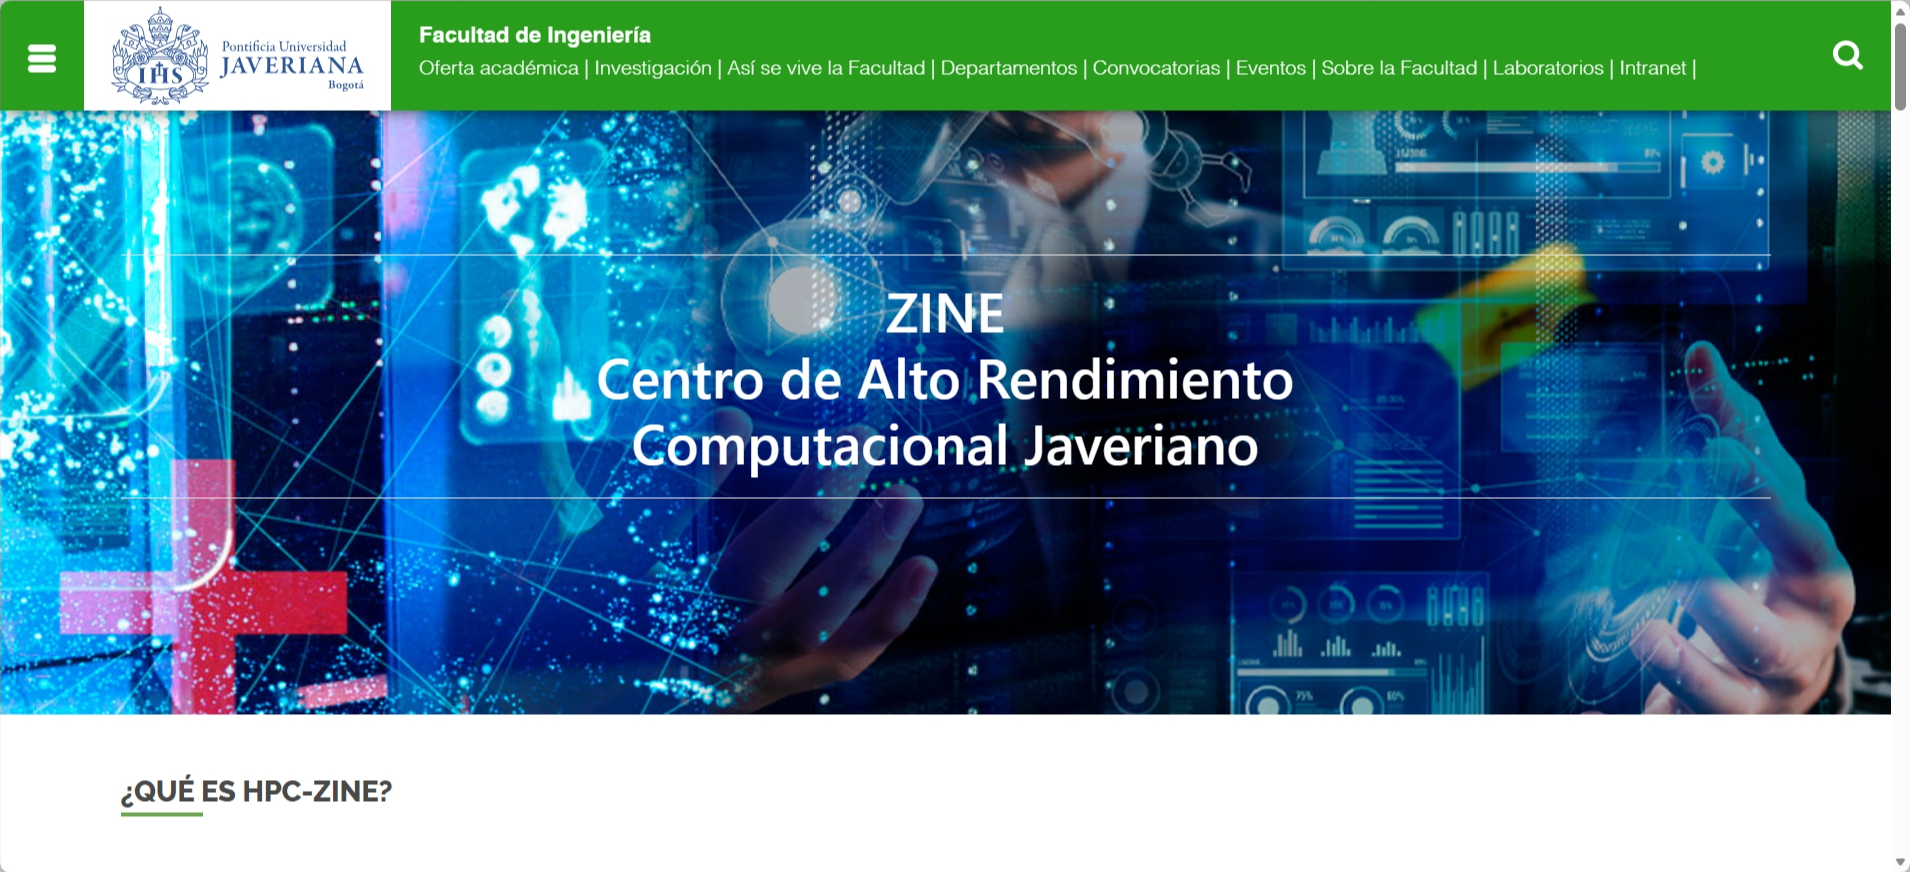
\includegraphics[width=0.95\textwidth]{images/ZINE/zine_pagina_oficial.png}
  \caption{Página oficial del Centro de Alto Rendimiento Computacional ZINE.}
  \label{fig:zine_web}
\end{figure}

\section{¿Por qué nace ZINE?}
En la investigación moderna aparecen problemas que, por su tamaño o complejidad, tardan demasiado tiempo si se ejecutan en un computador convencional. Ejemplos típicos incluyen simulaciones y análisis intensivos de datos, como el estudio de escenarios climáticos, el comportamiento de sistemas físicos, el análisis de series de tiempo o el trabajo con grandes volúmenes de información. En ese contexto, la computación de alto rendimiento (HPC, por sus siglas en inglés) permite reducir tiempos de cálculo al distribuir el trabajo entre múltiples procesadores y recursos especializados. \cite{pesquisa_zine_2012}

ZINE nació como respuesta a esa necesidad transversal: brindar a investigadores de distintas disciplinas una infraestructura capaz de ejecutar simulaciones y análisis de datos que requieren alta capacidad de cómputo y almacenamiento. En la descripción institucional del centro se indica que su creación se originó en las necesidades de investigadores que requieren simular o analizar datos, y que la infraestructura se encuentra alojada en el Datacenter de la Universidad para garantizar continuidad del servicio. \cite{zine_oficial}

Además de atender el reto tecnológico, ZINE se concibió como una iniciativa que promueve cooperación entre investigadores y grupos (internos y externos) alrededor de la supercomputación y tecnologías asociadas, con el objetivo de impulsar la adopción de HPC como herramienta científica. \cite{zine_oficial}

\section{¿Para qué es ZINE?}
ZINE es un servicio académico y científico orientado a apoyar la investigación y la docencia mediante capacidad de procesamiento y almacenamiento. Su misión institucional se expresa como la provisión de servicios de procesamiento y almacenamiento de información para apoyar procesos académicos de investigación y docencia. \cite{zine_oficial}

En términos simples, ZINE sirve para:
\begin{itemize}
  \item \textbf{Acelerar cálculos complejos:} reducir tiempos de ejecución de simulaciones y análisis.
  \item \textbf{Habilitar trabajos que no caben en equipos personales:} por volumen de datos, duración o requerimientos de cómputo.
  \item \textbf{Acompañar a los usuarios:} formación y asesoría para usar adecuadamente la infraestructura.
  \item \textbf{Fomentar colaboración:} conectar capacidades técnicas con necesidades de diferentes áreas del conocimiento.
\end{itemize}

La plataforma está enfocada en soportar trabajos de alto volumen asociados con áreas como Big Data, Machine Learning e Inteligencia Artificial, y en general con problemas que requieren modelar o simular escenarios complejos. \cite{perfiles_capacidades_zine}

\section{Servicios internos del ZINE en la Universidad Javeriana}
De acuerdo con la caracterización institucional, el HPC-ZINE pone a disposición de investigadores, docentes y estudiantes una infraestructura tecnológica para ejecutar trabajos de alto volumen y apoyar procesos de simulación y análisis en múltiples áreas. \cite{perfiles_capacidades_zine}

A nivel interno (comunidad Javeriana), los servicios suelen materializarse en cuatro componentes principales:

\subsection*{1) Infraestructura de cómputo y almacenamiento}
ZINE ofrece recursos para ejecutar cargas de trabajo intensivas y almacenar información asociada a los proyectos. Estos recursos se orientan a tareas como simulación, análisis y procesamiento de grandes volúmenes de datos. \cite{zine_oficial,perfiles_capacidades_zine}

\subsection*{2) Casos de uso en diferentes disciplinas}
Los recursos se emplean para simular y modelar escenarios, por ejemplo:
\begin{itemize}
  \item \textbf{Escenarios físicos:} predicción del estado del tiempo, análisis de estructuras mecánicas.
  \item \textbf{Escenarios biológicos:} análisis de secuencias (p.\,ej., ADN) y fenómenos de interés en ciencias de la vida.
  \item \textbf{Escenarios económicos y de datos:} análisis de series de tiempo y problemas de ciencia de datos e ingeniería.
\end{itemize}
\cite{perfiles_capacidades_zine}

\subsection*{3) Capacitación para el uso adecuado del HPC}
Dado que estas plataformas requieren preparación, se enfatiza la formación. Como ejemplo institucional de entrenamiento, se publican cursos de manejo de la infraestructura, incluyendo temas de acceso, uso de un gestor de tareas (por ejemplo, HTCondor) y envío de trabajos. \cite{curso_hpc_python}

\subsection*{4) Acompañamiento y asesoría técnica}
Además de la infraestructura, se destaca el acompañamiento a los investigadores para que puedan utilizar los recursos de manera efectiva en sus proyectos. \cite{perfiles_capacidades_zine,pesquisa_zine_2012}

\section{Servicios a investigadores externos}
ZINE no se limita a la comunidad interna. En su información institucional se indica que los servicios pueden ser requeridos por entidades externas que necesiten análisis y simulación de grandes cantidades de datos o simulación extensiva de modelos de aprendizaje, entre otros usos. \cite{zine_oficial}

En el portafolio de “Servicios externos” de la Facultad de Ingeniería, ZINE se presenta como una solución de cómputo de alto desempeño que ofrece recursos computacionales, capacitación y acompañamiento en proyectos de investigación, docencia, análisis y simulación para el sector académico y productivo. \cite{servicios_externos_zine}

De forma concreta, para usuarios externos se describen líneas de servicio como:
\begin{itemize}
  \item Capacitación y formación para el uso adecuado de infraestructura HPC.
  \item Asesoramiento para desplegar herramientas de analítica de datos e inteligencia artificial sobre HPC.
  \item Despliegue/uso de infraestructura alojada en Datacenter (se menciona Tier 2/3 en el portafolio).
  \item Almacenamiento de altos volúmenes de información, con énfasis en soberanía de los datos.
\end{itemize}
\cite{servicios_externos_zine}

Finalmente, desde una perspectiva institucional de colaboración académica, se ha indicado que, mediante proyectos interinstitucionales, investigadores y docentes de otras universidades pueden beneficiarse de este tipo de infraestructura. \cite{pesquisa_zine_2012}